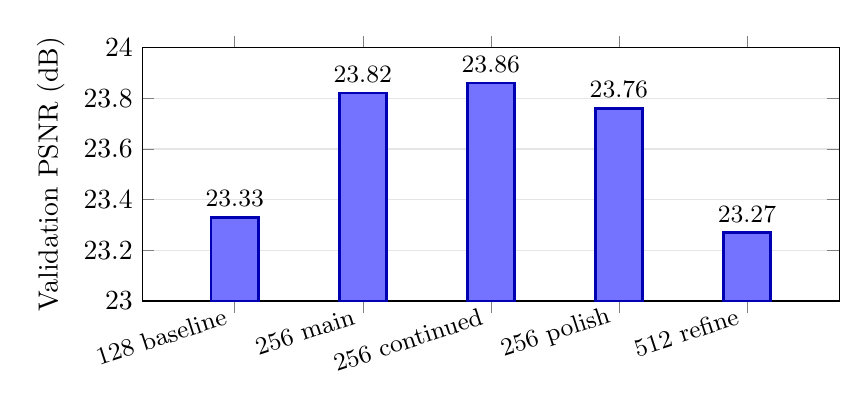
\begin{tikzpicture}
\begin{axis}[
    width=0.86\linewidth,
    height=4.8cm,
    ymin=23.0,
    ymax=24.0,
    ymajorgrids=true,
    grid style={black!10},
    symbolic x coords={128 baseline,256 main,256 continued,256 polish,512 refine},
    xtick=data,
    x tick label style={rotate=18,anchor=east,font=\small},
    ylabel={Validation PSNR (dB)},
    nodes near coords,
    nodes near coords style={font=\small},
    every axis plot/.append style={line width=0.9pt},
    bar width=17pt,
    ybar,
    enlarge x limits=0.18,
]
\addplot[fill=blue!55,draw=blue!70!black] coordinates {
    (128 baseline,23.33)
    (256 main,23.82)
    (256 continued,23.86)
    (256 polish,23.76)
    (512 refine,23.27)
};
\end{axis}
\end{tikzpicture}
